\section{Problema 2: Horizontes lejanos}

\subsection{Presentaci\'on del problema}
%aca ponemos una interpretacion de lo que nos pide el enunciado y algunas aclaraciones de como vamos a encarar el problema.
Dado un conjunto de rectángulos en un plano, todos apoyados sobre una linea recta horizontal, como en las siguientes figuras, se pide eliminar las líneas que colisionen con algún otro rectángulo, donde colisionar también es sólamente ``tocar'' otra línea.
\begin{figure}[ht]
	\begin{minipage}[t]{0.5\linewidth}
		\centering
		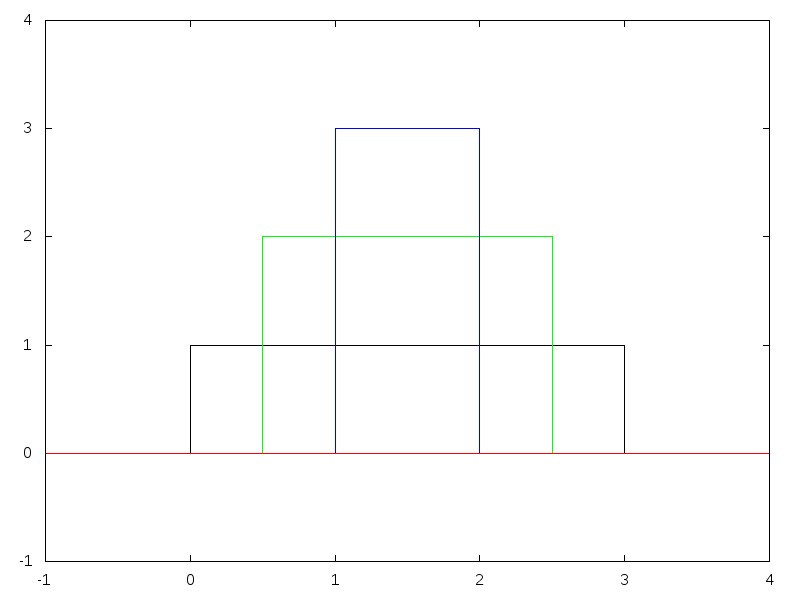
\includegraphics[width=\textwidth]{p1_ej1_pre.jpg}
		\caption{Con colisión total}
		\label{fig:p1_ej1_pre}
	\end{minipage}
	\begin{minipage}[t]{0.5\linewidth}
		\centering
		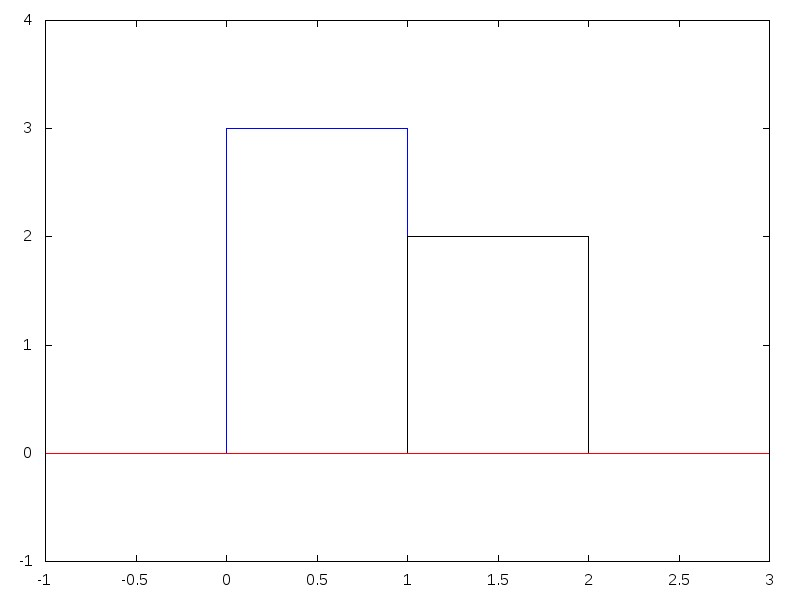
\includegraphics[width=\textwidth]{p1_ej2_pre.jpg}
		\caption{Sólo se tocan los bordes}
		\label{fig:p1_ej2_pre}
	\end{minipage}
\end{figure}

\noindent Así, tras ejecutar el algoritmo, el resultado para los ejemplos anteriores sería:

\begin{figure}[ht]
	\begin{minipage}[t]{0.5\linewidth}
		\centering
		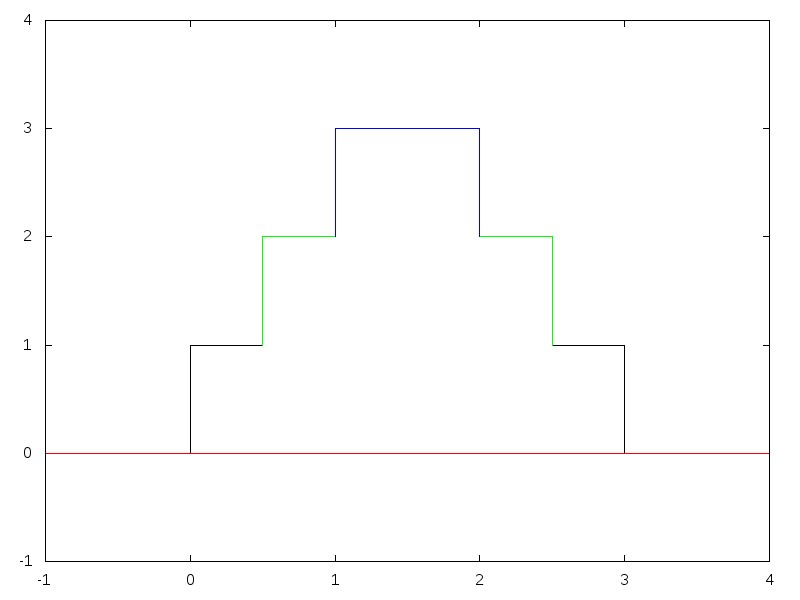
\includegraphics[width=\textwidth]{p1_ej1_post.jpg}
		\caption{Resultado con colisión total}
		\label{fig:p1_ej1_post}
	\end{minipage}
	\begin{minipage}[t]{0.5\linewidth}
		\centering
		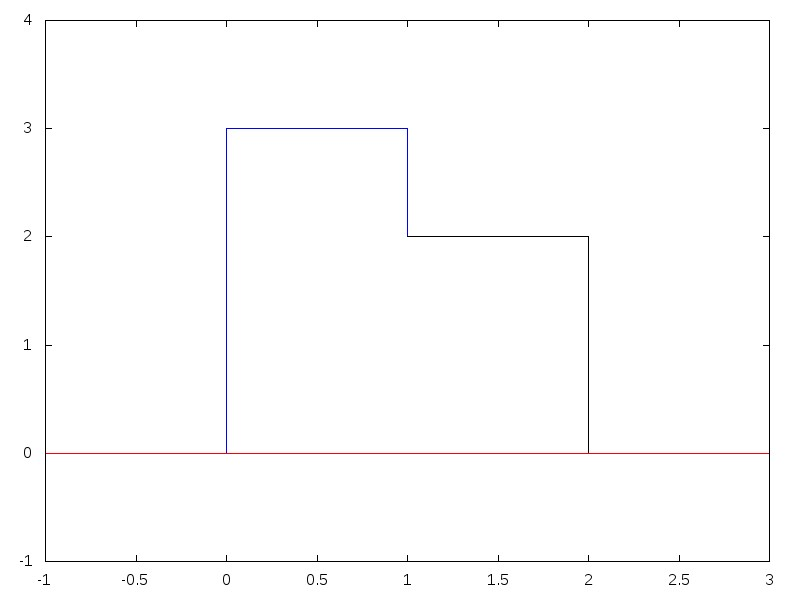
\includegraphics[width=\textwidth]{p1_ej2_post.jpg}
		\caption{Resultado cuando sólo se tocan los bordes}
		\label{fig:p1_ej2_post}
	\end{minipage}
\end{figure}

Como requerimiento adicional, el algoritmo para $n$ rectángulos debe tener una complejidad temporal estrictamente menor que $O(n^2)$.

\subsection{Resoluci\'on}
\subsubsection{Algoritmo}
%aca ponemos una descripcion de nuestro algoritmo, presentamos la variables las estructuras y decimos que hacemos.
COMPLETAR

\subsubsection{Pseudoc\'odigo}
%aca va el pseudocodigo del problema.
\begin{algorithm}
\begin{algorithmic}
	\STATE input: $edificios$
%	\STATE $eventos$ = parseEdificios($edificios$)
	\WHILE{quedan edificios}
		\IF{empieza edificio}
			\STATE registro el edificio como abierto
			\IF{altura del edificio es mayor a la del contorno}
				\STATE agrego la altura del edificio al contorno
			\ENDIF 
		\ELSE
			\STATE saco al edificio de los abiertos
			\IF{este edificio le daba la altura al contorno}
				\STATE agrego la altura del edificio abierto que le siga en altura al contorno
			\ENDIF
		\ENDIF
	\ENDWHILE
	
	\RETURN contorno
\end{algorithmic}
\end{algorithm}

\subsection{Demostraci\'on}
%aca va la demostracion formal del problema refiriendonos al pseudocodigo o redefiniendo variables (definir todas las cosas de las que vamos a hablar).

\subsection{An\'alisis de complejidad}
%aca decimos cuanto cuesta cada parte del algoritmo y damos un valor final de la complejidad del algoritmo, ej O(logn).

\subsection{Test de complejidad}
%aca van los graficos y todos los testeos que hagamos para probar que en la practica el algoritmo cumple la complejidad que propusimos en el punto anterior

\subsection{Testing}
%aca ponermos todos nuestros casos bordes, como actua nuestro algoritmo en los casos particulares.































